\documentclass[oneside]{scrbook}
\KOMAoptions{fontsize=11pt, paper=a4}     
\KOMAoptions{DIV=13}                      

\usepackage[utf8]{inputenc}               
\usepackage[T1]{fontenc}                  
\usepackage[autostyle=true]{csquotes}     
\usepackage[varg]{txfonts}  			  %	Times-like fonts in support of mathematics
\usepackage{siunitx}   	  				  
\usepackage{enumitem}				      %	extra enumerate options

\renewcommand{\familydefault}{\rmdefault} % font to sans serif

%import external graphics and where to find these
\usepackage{graphicx}					  
\graphicspath{{figs/}}

\RequirePackage[backend=biber, style=numeric]{biblatex}
\addbibresource{refs.bib}

\usepackage{hyperref}
\RequirePackage[all]{hypcap}

\usepackage{amsmath}
\usepackage{physics}
\usepackage{mathtools}
\usepackage{braket}
\usepackage{slashed} % feynman slash notation
\usepackage{simplewick} % wick contraction
% \usepackage{tikz-feynman} % feynman diagrams

%restart footnotes every page
\usepackage{perpage}
\MakePerPage{footnote}
%symbols for footnotes
\usepackage[symbol]{footmisc}
\renewcommand{\thefootnote}{\fnsymbol{footnote}} % footnote mark with special symbols

% toprule and etc.
\usepackage{booktabs}

%%%%%%%%%%%%%%%%%%%%%%%%%% NEW COMMAND SECTION %%%%%%%%%%%%%%%%%%%%

%define equal
\newcommand{\defeq}{\vcentcolon =} 
\newcommand{\eqdef}{= \vcentcolon}
\newcommand{\euler}{\mathrm{e}}

%Lagrange density
\newcommand{\lag}{\mathcal{L}} 
%Hamiltonian density
\newcommand{\ham}{\mathcal{H}}

%identity matrix
\usepackage{dsfont}
\newcommand{\id}{\mathds{1}}

\newcommand{\vecnab}{\pmb{\nabla}}
\newcommand{\vecx}{\pmb{x}}
\newcommand{\vecy}{\pmb{y}}
\newcommand{\veck}{\pmb{k}}
\newcommand{\vecp}{\pmb{k}}
\newcommand{\N}{\mathbb{N}}
\newcommand{\R}{\mathbb{R}}
\newcommand{\C}{\mathbb{C}}
\newcommand{\D}{\mathcal{D}}
\newcommand{\M}{\mathcal{M}}
\newcommand{\sm}{Standard Model }
\newcommand{\diag}{\text{diag}}
\newcommand{\sgn}{\text{sgn}}

%%%%%%%%%%%%%%%%%%%%%%%%%%%%% SETTINGS %%%%%%%%%%%%%%%%%%%%%%%%%%%%%%%%%%%%

\numberwithin{equation}{section}

%%%%%%%%%%%%%%%%%%%%%%%%%%%%%%%%%%%%%%%%%%%%%%%%%%%%%%%%%%%%%%%%%%

\title{Advanced Quantum Field Theory}
\author{Chenhuan Wang}
\date{\today}
\begin{document}
\maketitle
\tableofcontents

\chapter{Renormalisation and UV cutoffs}
see Peskin

\chapter[Path Integrals and Gauge Fields]{Path Integrals and Gauge Fields\footnote{see also in  Peskin and Schroeder Ch 9.1,  Ryder Ch 5.1, L.S.Brown Ch1 1-3}}

\section{Reminder: Path integrals in Quantum Mechanics}
Transition amplitude is given by 
\begin{align}
   \braket{x_b | \euler^{-iH(t_b - t_a)} | x_a}_{S} = \braket{x_b, t_b | x_a, t_a}_{H} 
\end{align}
Here we denotes the Schrödinger picture states by ${}_S$ and Heisenberg picture states by ${}_H$.

\begin{align}
   \ket{x_a, t_a} &= \euler^{iHt_a} \ket{x_a} \\
   \hat{H}_a (t_a) &= \euler^{iHt_a} \hat{x}_S \euler^{-iHt_a} \\
   \hat{x}_H(t_a) \ket{x_a, t_a} &= \euler^{iHt_a} \hat{x}_s \ket{x_a} = \euler^{iHt_a} x_a \ket{x_a}  \notag\\
                                 &= x_a \euler^{iHt_a} \ket{x_a} = x_a \ket{x_a, t_a}
\end{align}
We are looking at time evolution in position space.

It can be calculated directly for free particle with Hamiltonian $H = H_0 = \frac{\hat{p}^2}{2m}$

\begin{align}
   \braket{x_b | \euler^{-i \frac{\hat{p}^2}{2m}(t_b - t_a)} | x_a} = \sqrt{\frac{m}{2\pi i (t_b - t_a)}} \euler^{i(x_b - x_a)^2 \frac{m}{2(t_b - t_a)}}
\end{align}
We are going to insert $1 = \int \dd[3]{p} \ket{p}\bra{p}$ and use $\braket{x | p}$ is the plane wave

For general Hamiltonian $H = H_0 + V$ and $ \left[ H_0, V \right] \neq 0 $ the procedure is as following
\begin{itemize}
   \item divide $t$ into $N$ small intervals $t = N\cdot \epsilon$
   \item use Lie-Kato-Trotter product formula
      \begin{align}
         \euler^{A+B} = \lim_{N \rightarrow 0} \left( \euler^{A/N} \euler^{B/N} \right)^N \quad A, B \in GL(n, \C)
      \end{align}
\end{itemize}

Then we get a functional for path $x(t')$
\begin{align}
   \braket{ x_b | \euler^{-iH(t_b - t_a)}| x_a} = \int \mathcal{D}x \euler^{i S[x] / \hbar}
   \shortintertext{with $S[x] = \int_{t_a}^{t_b} \dd{t'} \left[ \frac{m}{2} \dot{x}(t') - V(x(t')) \right]$} \notag
\end{align}

\paragraph{Definition} (integration measure) 
\begin{align}
   \mathcal{D}x = D \left[ x(t) \right] = \lim_{N \rightarrow \infty} \left( \frac{mN}{2\pi i \Delta t} \right)^{N/2} \dd{x(t_1)} \dots \dd{x(t_{N-1})}
\end{align}
with $\Delta t = (t_b - t_a)/N$

Pictorially we sum over all paths (i.e.~amplitudes). Remember the superposition principle in quantum mechanics!

Classical path comes from Hamilton principle $\delta S = 0$
\begin{align}
   \left.\frac{\delta S[x]}{\delta x(t)} \right|_{x=x_{cl}} = 0
\end{align}

Classical path dominates the transition probability in the limit $\hbar \rightarrow 0$. It is the contribution with fewest oscillations in the path integral. Others interfere destructively (averaged out). This is essentially stationary phase approximation.

\paragraph{Example} (harmonic oscillation)
\begin{align}
   L = \frac{m}{2} \left( \dot{x}^2 - \omega^2 x^2 \right)
\end{align}
Then the classical path obeys the equation of motion
\begin{align}
   \ddot{x}_{cl}(t) + \omega^2 x_{cl}(t) = 0
\end{align}

Split a general path into classical and fluctuations $x(t) = x_{cl}(t) + y(t)$. The action turns into
\begin{align*}
   S[x] = S[x_{cl}] + \underbrace{\int \dd{t} \frac{\delta s}{ \delta x(t)} |_{x=x_{cl}}y(t)}_{=0} + \frac{1}{2} \int \dd{t} \int \dd{t'} \frac{\delta^2 S}{\delta x(t) \delta x(t')}|_{x=x_{cl}} y(t) y(t') + \dots
\end{align*}

Then we can factor out the classical path contribution in transition probability
\begin{align*}
   \braket{ x_b | \euler^{-iHT} | x_a } = \int \mathcal{D}x \euler^{\frac{i}{\hbar} S[x]} =  \euler^{\frac{i}{\hbar} S[x_a]} \int \mathcal{D}x \euler^{\frac{i}{\hbar} S[y]}
\end{align*}
The integral is to sum over fluctuations around the classical path. Ideally suited to treat fluctuations (quantum and thermal). The explicit calculation for harmonics oscillator can be found in AQT course.

\paragraph{Physical Interpretation} the transition probability is the propagator
\begin{align}
   \braket{x_b | \euler^{-iH(t_b - t_a)} | x_a} = U (x_b t_b; x_a t_a)
\end{align}

Superposition principle takes the form
\begin{align*}
   \psi(x_b, t_b) &= \braket{x_b | \psi(t_b) } = \braket{x_b | \euler^{-iHt_b} | \psi} \\
                  &= \int \dd{x_a} \braket{x_b | \euler^{-iH(t_b - t_a)}| x_a } \braket{x_a| \euler^{-iHt_a} | \psi} \\
                  &= \int \dd{x_a} U(x_b t_b; x_a t_a) \underbrace{\braket{x_a | \psi(t_a)}}_{\psi(x_a, t_a)} \\
\end{align*}

\section{Quantum Mechanical Path Integrals and External Forces}
\paragraph{Definition} (Time evolution operator) in path integral representation
\begin{align}
   U(x_b, t_b; x_a, t_a) &= \braket{x_b, t_b | x_a, t_a}\\
                       &= \int \D x(t) \euler^{iS[x]} \notag \\
                       &= \int \D x(t) \euler^{i\int^{t_b}_{t_a} \dd{t} L(x, \dot{x})} \notag
\end{align}

Add coupling to an external force (source) $f(t)$
\begin{align}
   L = L_0 + f(t) x(t)
\end{align}

\paragraph{Definition} (functional derivatives) with respect to $if(t)$
\begin{align}
   \frac{\delta}{\delta f(t)} \int \dd{t'} f(t') g(t') = g(t)
\end{align}

For a general functional of external forces
\begin{align}
   F[f] = \int \dd{t_1} K_1(f_1) f(t_1) + \frac{1}{2!} \int \dd{t_1} \dd{t_2} K_2(t_1, t_2) f(t_1) f(t_2)  + \dots
\end{align}
with the $K_n(t_1, \dots, t_n)$ totally symmetric in the arguments $t_1, \dots , t_n$, since antisymmetric contributions drop automatically upon integration. The functional derivatives is then
\begin{align}
   \frac{\delta F}{\delta f(t)} = K_1(t) + \int \dd{t_2} K_2 (t, t_2) f(t_2) + \frac{1}{2!} \int \dd{t_2} \dd{t_1} K_3(t, t_2, t_3) f(t_2) f(t_3) + \dots
\end{align}

Consider functional derivative of time evolution operator
\begin{align*}
   \frac{1}{i} \frac{\delta}{\delta f(t)} \braket{x_b, t_b | x_a, t_a}^f  
   &= \int \D x \exp(i \int^{t_b}_{t_a} \dd{t'}L_0) \frac{1}{i} \frac{\delta}{\delta f(t)} \exp(i\int^{t_b}_{t_a}\dd{t'}f(t')x(t')) \\
   &= \int \D x \, x(t) \exp(i\int^{t_b}_{t_a} \dd{t'} \left[ L_0 + f(t') x(t') \right] )
\end{align*}

To split the path integral into two parts, time before and after $t$ (superposition principle). $M$ steps before $t$ and $N-M-1$ steps after $t$. The integration over $x(t)$ is to sum over all possible positions at time $t$.
\begin{align*}
   \int^{t_b}_{t_a} \D x  = \int \dd{x(t)} \int^{t_b}_t \D x \int^t_{t_a} \D x
\end{align*}

Then
\begin{align*}
   \frac{1}{i} \frac{\delta}{\delta f(t)} \braket{x_b, t_b | x_a, t_a}^f  &= \int \dd{x(t)} \underbrace{\int \D x \exp(i \int^{t_b}_{t} \dd{t'} (L_0 + f x))}_{N-M-1 \text{ factor}} x(t) \underbrace{\int \D x \exp(i\int^{t_b}_{t_a} \dd{t'} (L_0 + fx))}_{M \text{ factor}} \\
                                                                        &= \int \dd{x(t)} \braket{x_b, t_b | x(t), t}^f x(t) \braket{x(t), t | x_a, t_a}^f
\end{align*}
Here $x(t)$ is an eigenvalue, not an operator, so we write $x(t) = \bar{x}$ with 
\begin{align*}
\int \dd{\bar{x}} \ket{\bar{x}, t} \bar{x} \bra{\bar{x}, t} = \int \dd{\bar{x}} \bar{x} \braket{\bar{x}, t | \bar{x}, t}  = x(t)
\end{align*}
the Heisenberg operator.

We get 
\begin{align}
   \frac{1}{i} \frac{\delta}{\delta f(t)} \braket{x_b t_b | x_a t_a}^f 
   = \braket{x_b, t_b | x(t) | x_a, t_a}
\end{align}

The functional derivative with respect to the external force $f(t)$ which couples to $x(t)$, to "insert" the operator $x(t)$ into the matrix element.

Now consider \textit{two} functional derivatives with $t_b \geq t, t' \geq t_a$
\begin{align}
   \frac{1}{i} \frac{\delta}{\delta f(t)} \frac{1}{i} \frac{\delta}{\delta f(t')} \braket{x_b, t_b | x_a, t_a}^f 
   = \int \D x \, x(t) x(t') \euler^{i\int^{t_b}_{t_a} \dd{t'} \left[ L_0 + f\cdot x \right]}
\end{align}

In general
\begin{align*}
   \frac{1}{i} \frac{\delta}{\delta f(t)} \frac{1}{i} \frac{\delta}{\delta f(t')} \braket{x_b, t_b | x_a, t_a}^f 
   &= \frac{1}{i} \frac{\delta}{\delta f(t)} \braket{ x_b, t_b | x(t') | x_a, t_a}^f \\
   &= \frac{1}{i} \frac{\delta}{\delta f(t)} \int \dd{\bar{x}'} \braket{ x_b, t_b | x(t') | \bar{x}', t}^f \bar{x}' \braket{\bar{x}', t' | x_a, t_a}^f \\
   &= \int \dd{\bar{x}'} \left(\frac{1}{i} \frac{\delta}{\delta f(t)} \braket{ x_b, t_b | x(t') | \bar{x}', t}^f \right) \bar{x}' \braket{\bar{x}', t' | x_a, t_a}^f  \\
   &\quad + \int \dd{\bar{x}'} \braket{ x_b, t_b | x(t') | \bar{x}', t}^f \bar{x}' \left(\frac{1}{i} \frac{\delta}{\delta f(t)}\braket{\bar{x}', t' | x_a, t_a}^f \right)
\end{align*}

Then transition amplitudes only depend on the time interval, where the external forces actually act
\begin{align*}
   \frac{1}{i} \frac{\delta}{\delta f(t)} \braket{x_b, t_b | \bar{x}', t'}^f &= 
   \begin{cases}
      \braket{x_b, t_b | x(t) | \bar{x}', t'}^f & t > t' \\
      0 & t < t'
   \end{cases} \\
   \frac{1}{i} \frac{\delta}{\delta f(t)} \braket{\bar{x}', t' | x_b, t_b   }^f &= 
   \begin{cases}
      0 & t > t' \\
      \braket{\bar{x}', t' | x(t) | x_b, t_b}^f & t < t'
   \end{cases}
\end{align*}

Eliminate $\bar{x}'$ integration as before
\begin{align}
   \frac{1}{i} \frac{\delta}{\delta f(t)} \frac{1}{i} \frac{\delta}{\delta f(t')} \braket{x_b, t_b | x_a, t_a}^f  
   = \braket{x_b, t_b | T \left[x(t), x(t') \right] | x_a, t_a}^f
\end{align}

This can be easily generalised
\begin{align}
   \frac{1}{i} \frac{\delta}{\delta f(t')} \frac{1}{i} \frac{\delta}{\delta f(t'')} \dots \braket{x_b, t_b | x_a, t_a}^f 
   &= \braket{x_b, t_b | T \left[ x(t') x(t'') \dots  \right] |x_a, t_a}^f \\
   &= \int \D x \, x(t') x(t'') \dots \exp(i\int^{t_b}_{t_a} \dd{t} \left( L_0(x, \dot{x}) + f(t) x(t) \right))
\end{align}

\paragraph{Interpretation} the addition of external force to the Lagrangian of a path integral produces a "generating functional" for a matrix element which contain time-ordered products of arbitrary many position operators. The functional derivative is just a trick to generate the matrix element in the propagator. This is called Schwinger source theory.

Now we can set $f=0$
\begin{align}
   \braket{x_b, t_b | T \left[ x(t') x(t'') \dots  \right] |x_a, t_a}^{f=0}
   = \int \D x x(t') x(t'') \dots \exp(i\int^{t_b}_{t_a}  L_0(x, \dot{x}) )
\end{align}
or in case of an arbitrary generating functional $F[x]$ 
\begin{align}
   \braket{x_b, t_b | T \left\{ F[x]  \right\} |x_a, t_a}^{f=0}
   = \int \D x F[x] \exp(i\int^{t_b}_{t_a}  L_0(x, \dot{x}) )
\end{align}
for example
\begin{align*}
   \braket{x_b, t_b | x_a, t_a}^f = \braket{ x_b, t_b | T \euler^{i\int^{t_b}_{t_a} \dd{t'} q(t') f(t')} | x_a, t_a}^{f=0}
\end{align*}

\section{Scalar Field Theories and Feynman Rules}
We are going to generalise the concept of path integral to field theories. Simplest example is a neutral (real) scalar field $\phi(x)$ coupled to an external classical "current"/source $j(x)$
\begin{align}
   \lag = \frac{1}{2} \left( \partial_\mu \phi \right)^2 - \frac{1}{2} m^2 \phi^2 + \phi j(x) = \lag_0 + \phi(x) j(x)
\end{align}

Proceed along the lines of quantum mechanical path integral with external forces
\begin{itemize}
   \item construct a generating functional
   \item using the functional-integral-representation derive expressions for the correlation functions $\stackrel{\sim}{=}$ Feynman rules
\end{itemize}

Sufficient to consider vacuum-to-vacuum amplitudes in the presence of $j(x)$. Consider $t_a = -\infty(1-i\epsilon)$, $t_b = +\infty(1-i\epsilon)$ and $j(x) = 0$ for $t \mapsto \pm \infty$
\begin{align*}
   \braket{0 | 0}^j = \int \D x \, \phi(x) \exp(i\int \dd[4]{x}\lag(\phi, \partial_\mu \phi))
\end{align*}
where $\D \phi(x)$ in the generalization $\D x \mapsto \D (\text{field})$

Compute $\braket{0|0}^j$ (exact for a free field theory). First to solve with classical action
\begin{align*}
   \delta \int \dd[4]{x} \left[ \frac{1}{2} \left( \partial_\mu \phi_{cl} \right)^2 - \frac{1}{2} m^2 \phi^2_{cl} + \phi_{cl}j \right] &= 0\\\
   \left( \partial^2 + m^2 \right) \phi_{cl}(x) &= j(x)
\end{align*}

Solution 
\begin{align}
   \phi_{cl}(x) = i \int \dd[4]{y} D_F(x-y) j(y)
\end{align}
since Feynman-propagator is the Green's function of the KG operator.
\begin{align}
   \left( \partial^2 + m^2 \right) D_F(x-y) = -i \delta^{(4)}(x-y)
\end{align}

To define the "fluctuation" field $\phi'(x)$ via $\phi(x) = \phi_{cl}(x) + \phi'(x)$. Then the Lagrangian is
\begin{align*}
   \lag &= \frac{1}{2} \left( \partial_\mu \phi_{cl} + \partial_\mu \phi'\right)^2 -  \frac{m^2}{2} \left( \phi_{cl} + \phi' \right)^2 + \left( \phi_{cl} + \phi' \right) \cdot j(x) \\
        &= \lag_{cl} + \lag' + \left[ (\partial_\mu \phi_{cl}) (\partial^\mu \phi') - m^2 \phi_{cl} \phi' + j\phi \right] 
\end{align*}
after integration by parts and using equation of motion the last part vanishes. Then $\phi'$ (per construction) is a free field. Thus
\begin{align}
   \braket{0 | 0 }^j = \int \D \phi' \exp(i\int \dd[4]{x} (\lag_{cl} + \lag'))
   = \euler^{iS_{cl}} \braket{0 | 0}^{j=0}
\end{align}

On the other hand, $iS_{cl}$ can be rewritten as
\begin{align*}
   iS_{cl} &= i \int \dd[4]{x} \left[ \frac{1}{2} - \frac{m}{2} \phi_{cl}^2 + \phi_{cl} j \right] \\
           &= i \int \dd[4]{x} \bigg[ -\frac{1}{2} \phi_{cl} \underbrace{\left( \partial^2 + m^2 \right)\phi_{cl}}_{=j \;\text{from e.o.m.}} + \phi_{cl} j \bigg] \\
           &= \frac{i}{2} \int \dd[4]{x} \phi_{cl}(x) j(x) \\
           &= -\frac{1}{2} \int \dd[4]{x} \dd[4]{y} j(x) D_F(x-y) j(y)
\end{align*}

\paragraph{Definition} (generating functional) in the free scalar field theory
\begin{align}
   W_0[j] &= \frac{Z[j]}{Z[j=0]} = \frac{\braket{0 | 0}^j}{\braket{0 | 0}^{j=0}} \notag\\
            &= \exp(-\frac{1}{2} \int \dd[4]{x}\dd[4]{y} j(x) D_F(x-y) j(y))
\end{align}

Connection to the S-matrix
\begin{align}
   S &= U(-\infty, \infty) \notag\\
     &= \lim_{t_i \mapsto -\infty(1-i\epsilon)}\lim_{t_f \mapsto +\infty(1-i\epsilon)} T \exp(-i\int^{t_f}_{t_i} \dd{t} \ham_{int} (t)) \notag\\
   &= T \exp(-i\int \dd[4]{x}\ham_{int} (x)) \notag\\
   &= T \exp(i\int \dd[4]{x} \phi(x) j(x)) \notag\\
   &= T \sum_{n=0}^{\infty} \frac{i^n}{n!} \int \dd[4]{x_1} \dots \dd[4]{x_n} j(x_1) \dots j(x_n) \phi(x_1) \dots \phi(x_n) \notag\\
   \braket{0 | S | 0} &= \sum_{n=0}^{\infty} \frac{i^n}{n!} \int \dd[4]{x_1} \dots \dd[4]{x_n}  j(x_1) \dots j(x_n)G_n^0 (x_1, \dots, x_n)
\end{align}
where $G^0_n(x_1, \dots, x_n) = \braket{0 | T [\phi(x_1) \dots \phi(x_n)]| 0}$ the n-point-Green's function of the free scalar field theory.

We can calculate the Green's function as for the quantum mechanical path integral with external forces via functional derivatives of the generating functional
\begin{align}
   W_0[j] = \frac{\int \D \phi \exp(i\int \dd^4 x (\lag_0(\phi, \partial_\mu \phi)+\phi j))}{\int \D \phi \exp(i\int \dd^4 x (\lag_0(\phi, \partial_\mu \phi)))}
\end{align}

\begin{align}
   G_n^0 (x_1,\dots, x_n) &= \frac{1}{i} \frac{\delta}{ \delta j(x_1)} \dots \frac{1}{i} \frac{\delta}{ \delta j(x_n)} W_0[j] |_{j=0} \notag \\
                          &= \frac{\int \D \phi \exp(i\int \dd^4 x (\lag_0(\phi, \partial_\mu \phi)) )\phi(x_1) \dots \phi(x_n) }{\int \D \phi \exp(i\int \dd^4 x (\lag_0(\phi, \partial_\mu \phi)))} \notag \\
                          &= \braket{0 | T \phi(x_1) \dots \phi(x_n) | 0}
\end{align}

The central result here is that these three things are closely related: S-matrix $\leftrightarrow$ Green's function $\leftrightarrow$ Path integral

\chapter{The Renormalization Group}
\section[The Wilsonian Renormalization Group]{The Wilsonian Renormalization Group\footnote{P \& S, Ch 12.1}}
We will study influence of UV fluctuations more explicitly using UV cutoff $\Lambda$. It is difficult for gauge theories, but more intuitive for $\phi^4$.

Consider path integral with field vanishes in momentum space,
\begin{align*}
   Z[J] &= \int [\D \phi] \exp{i\int \dd[4]{x} (\lag + \phi J)} \\
        &= \prod_k \int \dd{\phi(k)}  \exp{i\int \dd[4]{x} (\lag + \phi J)}
\end{align*} 
We would like to separate out integration over modes with $|k| \leq \Lambda$. It is difficult in Minkowski space, since Minkowski "scalar product" is not positive semi-definite. So first perform Wick rotation to Euclidean space, where momentum cutoff $\Lambda$ is well defined. Euclidean path integral
\begin{align}
   \eval{Z_E[J]}_{J=0} &= \int [\D \phi]_\Lambda \exp{-\int \dd[d]{x_E} \left(\frac{1}{2} ( \partial \phi)^2 + \frac{1}{2} m^2 \phi^2 + \frac{\lambda}{4!}\phi^4 \right)}
\end{align}
Drop the subscript $E$ from now on. $m$ and $\lambda$ are bare parameters, there are no counter-terms yet. Dimension $d$ to keep discussion general.

Idea is to lower the cutoff $\Lambda$ somewhat, from $\Lambda \rightarrow b \Lambda$, with b a small positive number $ 0 < b < 1$. 
\paragraph{Define} \underline{low- and high-momentum modes} 
\begin{align}
   \tilde{\phi}(k) &= \begin{cases} \phi(k) & |k| \leq b \Lambda  \\ 0 &  |k| > b\Lambda \end{cases} \\
   \hat{\phi}(k) &= \begin{cases} 0 & |k| \leq b \Lambda \\ \phi(k) & b \Lambda < |k| \leq \Lambda \end{cases}
\end{align}
so that field can be decomposed into low-momentum modes and high-momentum modes.
\begin{align}
   \phi(k) = \tilde{\phi}(k) + \hat{\phi}(k) 
\end{align}
Rename low-momentum mode $\tilde{\phi}(k) = \phi(k)$.

In the path integral $[\D \phi]_{\Lambda} = [\D \phi]_{b \Lambda} [\D \hat{\phi}]$ and substitute $\phi \mapsto \phi + \hat{\phi}$ in the Lagrangian.
\begin{align*}
   Z &= \int [\D \phi]_{b \Lambda} \int [\D \hat{\phi}] \exp{ - \int \dd[d]{x} \left[\frac{1}{2} (\partial \phi + \partial \hat{\phi})^2 + \frac{m^2}{2}(\phi + \hat{\phi})^2 + \frac{\lambda}{4!} (\phi + \hat{\phi})^4 \right] } \\
     &=  \int [\D \phi]_{b \Lambda} \exp{- \int \dd[d]{x} \lag [\phi]} \int [\D \hat{\phi}] \exp{ - \int \dd[d]{x} \left[ \frac{1}{2} (\partial \hat{\phi})^2 + \frac{m^2}{2} \hat{\phi}^2 + \lambda \left(\frac{1}{6} \phi^3 \hat{\phi} + \frac{1}{4} \phi^2 \hat{\phi}^2 + \frac{1}{6} \phi \hat{\phi}^3 + \frac{1}{4!} \hat{\phi}^4 \right) \right]}
\end{align*}
Note that terms of order $\phi\hat{\phi}$ vanish! They would contribute to propagator-type terms, not have disjoint momentum support (different Fourier components orthogonal!)

Interaction terms of the form (double line for high momentum modes, single line for low momentum modes)
\begin{align*}
   \feynmandiagram[small, layered layout]{
      i1 -- v-- f1;
      i2 -- v-- f2;
   };\quad 
   \feynmandiagram[small, layered layout]{
      i1 -- v--[double] f1;
      i2 -- v-- f2;
   };\quad 
   \feynmandiagram[small, layered layout]{
      i1 -- v--[double] f1;
      i2 -- v--[double] f2;
   };\quad 
   \feynmandiagram[small, layered layout]{
      i1 --[double] v--[double] f1;
      i2 -- v--[double] f2;
   };\quad 
   \feynmandiagram[small, layered layout]{
      i1 --[double] v--[double] f1;
      i2 --[double] v--[double] f2;
   };
\end{align*}

After $\int \D \hat{\phi}$ path integral is carried out, the generating function should look like
\begin{align*}
   Z \stackrel{!}{=} \int [\D \phi]_{b \Lambda} \euler^{-\int \dd[d]{x} \lag_\text{eff}(\phi)}
\end{align*}
Now $\lag_\text{eff}$ only involves Fourier components with $|k| \leq b \Lambda$.

How does $\lag_\text{eff}$ look like?
\begin{align}
   \lag_\text{eff} = \lag(\phi) + \text{corrections}
\end{align}
The corrections are in order of $\lambda$. The correction terms compensate for the removal of high-momentum Fourier components/fluctuations in $\hat{\phi}$.

We are interested in large-ish cutoffs $\Lambda^2 \gg m^2$. Treat $m^2$ and $\lambda$ terms in the $\D \hat{\phi}$ path integral as perturbations. Leading propagator comes from
\begin{align*}
   \int \dd[d]{x} \lag_0 &= \int \dd[d]{x} \frac{1}{2} (\partial \hat{\phi})^2 \\
                         &= \int \frac{\dd[d]{k}}{(2\pi)^d} \frac{1}{2} \hat{\phi}^*(k) k^2 \hat{\phi}(k)
\end{align*}

The contraction is similar to a normal propagator 
\begin{align}
   \bcontraction{}{\hat{\phi}}{(k)}{\hat{\phi}} \hat{\phi} (k) \hat{\phi} (p) = \frac{\int \D \hat{\phi} \hat{\phi}(k) \hat{\phi} (p) \euler^{-\int \dd[d]{x} \lag}}{\int \D \hat{\phi} \euler^{-\int \dd[d]{x}\lag_0 }} \notag \\
   = \frac{1}{k^2} (2\pi)^d \delta^{(d)}(p + k) \hat{\theta}(k)  \label{math:phiphi}
   \shortintertext{where}
   \hat{\theta}(k) = \begin{cases} 1 & b \Lambda < |k| \leq \Lambda \\ 0 & \text{otherwise} \end{cases} \notag
\end{align}

Perturbations in $m^2$ and $\lambda$ are calculated expanding the exponential, using Wick's theorem with propagator from above. What corrections in $\lag_\text{eff}$ will the $\hat{\phi}$ field generate?

\paragraph{Tree level diagrams} 
Diagram with $\phi^3 \bcontraction{}{\hat{\phi}}{\phi^3}{\hat{\phi}} \hat{\phi} \phi^3 \hat{\phi}$
\begin{align*}
   \feynmandiagram[baseline=(v1.base), small, horizontal=v1 to v2, layered layout]{
      {i1[particle=\(p_1\)], i2[particle=\(p_2\)], i3[particle=\(p_3\)]} -- v1 --[double] v2 -- {f1[particle=\(p_1\)], f2[particle=\(p_2\)], f3[particle=\(p_3\)]};
   };
   \sim \frac{\lambda^2}{(p_1 + p_2+ p_3)^2} \hat{\theta} (p_1 + p_2 + p_3)
\end{align*}
does not contribute for $p_1, p_2, p_3 \ll \Lambda^2$. Similarly other tree-level diagrams won't contribute.

Consider $p_i = 0$ (external) for now!

\paragraph{Single $\hat{\phi}$ loop}
\begin{align*}
   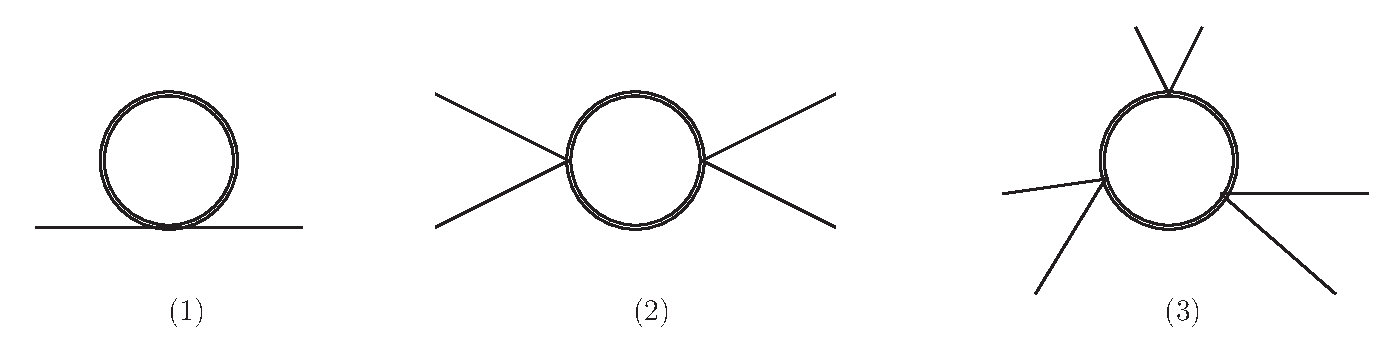
\includegraphics[width=0.8\linewidth]{./RG/1.eps}
\end{align*}

Calculate $(1)$ explicitly using equation (\ref{math:phiphi})
\begin{align*}
   (1) = -\frac{\lambda}{4}  \int \dd[d]{x} \phi^2 \bcontraction{}{\hat{\phi}}{}{\hat{\phi}} \hat{\phi} \hat{\phi} &=: - \frac{1}{2}\int \frac{\dd[d]{k_1}}{(2\pi)^d} \Delta m^2 \phi(k_1) \phi(-k_1)  \\
\end{align*}
in which 
\begin{align*}
   \Delta m^2 &= \frac{\lambda}{2} \int_{b \Lambda < |k| \leq \Lambda} \frac{\dd[d]{k}}{(2\pi)^d} \frac{1}{k^2} \\
              &= \frac{\lambda}{2} \frac{\Omega_d}{(2\pi)^d} \int_{b \Lambda}^\Lambda \dd{k} k^{d-3} \\
              &= \frac{\lambda}{(4\pi)^{d/2}} \frac{1}{\Gamma (d/2)} \frac{\Lambda^{d-2}}{d-2} (1- b^{d-2})
   \shortintertext{with $n$ dimensional solid angle $\Omega_d = 2 \pi^{d/2} / \Gamma(d/2)$. In $d=4$}
   \Delta m^2 &= \frac{\lambda}{16 \pi^2} \frac{\Lambda^2}{2} (1-b^2)
\end{align*}
 Remember $b < 1$ so $\Delta m^2 > 1$.

Second diagram give $- \frac{\Delta \lambda}{4!} \phi^4$ in effective Lagrangian. Setting external momenta to zero
\begin{align*}
   \Delta \lambda &= - 4! \frac{2}{2!} \left(\frac{\lambda}{4}\right)^2 \int \frac{\dd[d]{k}}{(2\pi)^d} \left( \frac{1}{k^2} \right)^2  \\
                  &= - \frac{3}{2} \lambda^2 \frac{2}{(4\pi)^{d/2} \Gamma(d/2)} \int_{b \Lambda}^{\Lambda} \dd{k} k^{d-5} \\
                  &= \frac{-3 \lambda^2}{(4\pi)^{d/2} \Gamma(d/2)} \frac{\Lambda^{d-4}}{d-4} (1-b^{d-4})  \\
                  &= - \frac{3 \lambda^2}{16 \pi^2} \ln( \frac{1}{b})
\end{align*}
It's negative since $0 < b < 1$!

If we set external momenta $p_i \neq 0$: Taylor expand in $p_i$,  it will generate interactions terms $(\partial \phi)^2 \phi^2$, $(\partial \phi)^4$, $\dots$.

Third diagram generates term $\sim \lambda^3 \phi^6$ (in $d=4$, $\propto \frac{\lambda^3 \phi^6}{\Lambda^2}$). Higher dimensional, non-renormalizable interactions are generated! We will see soon why it is not a real problem.

\paragraph{Comments}
\begin{itemize}
   \item Everything is finite, although being cutoff-dependent
   \item Is loop expansion $\frac{\lambda + \Delta \lambda}{4!} \phi^4$ valid?
      \begin{align*}
         \lambda + \Delta \lambda = \lambda \bigg[ 1- \underbrace{\frac{3\lambda}{16 \pi^2} \ln(1/b)}_{\ll 1} \bigg]
      \end{align*}
      Higher order ($N$ loops) will scale like $\lambda (\frac{\lambda}{16\pi^2} \ln(1/b))^N$. 
      \begin{align*}
         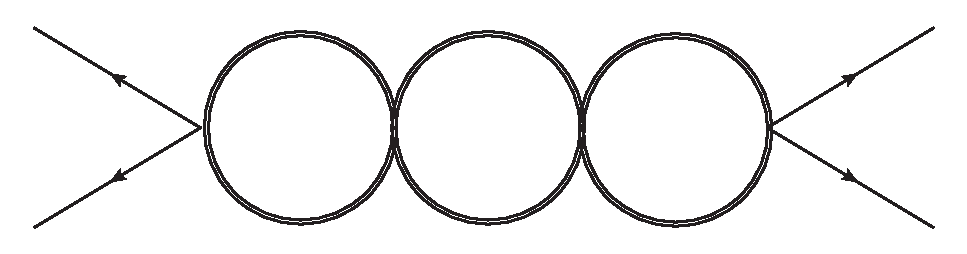
\includegraphics[width=0.4\linewidth]{./RG/2.eps} 
      \end{align*}
      It is even smaller corrections.
\end{itemize}

More careful comparison of $\lag $ and $ \lag_\text{eff}$
\begin{align*}
   Z &= \int [\D \phi]_{b \Lambda} \euler^{- \int \dd[d]{x} \lag_\eff} \\
   \lag_\text{eff} &= \frac{1}{2} (1 + \Delta Z) (\partial \phi)^2 + \frac{1}{2} (m^2 + \Delta m^2) \phi^2 + \frac{1}{4!} (\lambda + \Delta \lambda) \phi^4 + \Delta C ((\partial \phi)^2)^2 + \Delta \tilde{C} \phi^2 (\partial \phi)^2 + \Delta D \phi^6 + \dots
\end{align*}

Now rescale distances and momenta $k' = k / b$ or $x' = xb$. $k'$ in integrated up to $\Lambda$ (original cutoff).
\begin{align*}
   \int \dd[d]{x} \lag_\eff &= \int \dd[d]{x'} b^{-d} \bigg[ \frac{1}{2} (1+\Delta z) b^2 (\partial' \phi)^2 + \frac{1}{2} (m^2 + \Delta m^2)\phi^2 \\
      &+ \frac{1}{4!} (\lambda + \Delta \lambda) \phi^4 + \Delta C b^4 (\partial \phi)^4 + \tilde{\Delta C}b^2 (\partial' \phi)^2 \phi^2 + \Delta D \phi^6 + \dots \bigg]
\end{align*}
Now rescale the fields  
\begin{align*}
  \phi' = \sqrt{b^{2-d} (1+ \Delta Z)} \phi 
\end{align*}
to obtain canonical kinetic term
\begin{align*}
      \int \dd[d]{x} \lag_\eff &= \int \dd[d]{x'} \left[ \frac{1}{2} (\partial' \phi')^2 + \frac{1}{2} m'^2 \phi'^2 + \frac{1}{4!} \lambda' \phi'^4 + C' (\partial' \phi')^4 + \tilde{C}' (\partial' \phi')^2 \phi'^2 + D' \phi'^6 \right]
\end{align*}
with the scaled variables
\begin{align*}
   m'^2 &= \frac{m^2 + \Delta m^2}{b^2(1+\Delta Z)} \\
   \lambda' &= \frac{\lambda + \Delta \lambda}{b^{4-d} (1+ \Delta Z)^2} \\
   C' &= b^d \frac{C+ \Delta C}{(1+\Delta Z)^2} \\
   \tilde{C}' &= b^{d-2} \frac{\tilde{C} + \Delta \tilde{C}}{(1+\Delta Z)^2} \\
   D' &= b^{2d-6} \frac{D+ \Delta D}{(1+\Delta Z)^3}
\end{align*}
Even if we had $C = \tilde{C} = D = 0$ initially, it would apply as well.

So combination of integrating out degree of freedom and rescaling leads to transformation of $\lag$ (with identical $Llamba$). $\lag$ characterized by set of coupling constants 
\begin{align*}
  (m^2, \lambda, C, \tilde{C}, D, \dots) \mapsto (m'^2, \lambda', C', \tilde{C}', D', \dots) 
\end{align*}

This operation can be repeated, make it infinitesimal $ b \mapsto 1 - db$, so that it's continuous. Transformation in space of all possible Lagrangians.

Study trajectory or flows leads to Renormalization Group. It is not really a group, rather a semi-group, as transformation of "integrating-out" high-momentum degree of freedom is not invertible.

Two possible ways to perform calculations of correlation functions for $|p_i| \ll \Lambda$ 
\begin{itemize}
   \item use original $\lag$, high-momentum fluctuations in loops
   \item use $\lag_\eff$ high-momentum fluctuations have been absorbed in new coupling constants. Already at tree-level. Essentially it is effective field theory.
\end{itemize}

\paragraph{Renormalization Group (RG) in Detail}
Consider $\lag$ near the free theory $m^2 = \lambda =C = \tilde{C} = D = \dots = 0$
\begin{align*}
   \lag_0 = \frac{1}{2} (\partial \phi)^2
\end{align*}
$\lag_0$ is unchanged under the RG flow. It is fixed point.

Near $\lag_0$, only consider terms \underline{linear} in perturbation. Neglect $\Delta m^2 (\propto \lambda), \Delta \lambda (\propto \lambda^2), \Delta Z (\propto \lambda^2), \Delta C, \Delta \tilde{C} (\propto \lambda^2), \Delta D (\propto \lambda^3)$. Then simply have 
\begin{align*}
   m'^2 &= m^2 b^{-2} \\
   \lambda' &= \lambda b^{d-4} \\
   \tilde{C}' &= \tilde{C} b^{d-2} \\
   C' &= C b^d \\
   D' &= D b^{2d-6}
\end{align*}

Since $0 < b < 1$, behaviours are classified as following
\begin{itemize}
   \item \underline{relevant} term grows with RG, 
   \item \underline{marginal} term in $d=4$ unchanged  (higher orders unimportant)
   \item \underline{irrelevant} term diminished in RG flow
\end{itemize}

This can actually be seen directly from dimensional analysis. Operator with $N$ fields $\phi$ and $M$ derivatives scales as 
\begin{align*}
   C'_{N, M} &= b^{N(d/2 - 1) + M - d} C_{N, M} \\
             &= b^{d_{N, M} - d} C_{N, M}
\end{align*}
with $d_{N,M}$ mass dimension of the operator.

Note: relevant/marginal/irrelevant terms correspond to super-renormalizable/renormalizable/non-renormalizable interactions.

One can understand evolution of couplings near a fixed point from dimensional analysis! Near fixed point, arbitrary complicated $\lag$ reduces to a finite number of renormalizable term! (Only near fixed point!)

Illustrate RG flow for $\phi^4$ in 3 cases
\begin{itemize}
   \item \underline{$d > 4$} only mass term is relevant, everything else irrelevant. Only $m^2$ grows, since $m'^2 = m^2 b^{-2n}$ after $n$ iterations. Ultimately $m'^2 \sim \Lambda^2$. Integrate complete momentum range between $\Lambda$ and the effective mass $m'$.
   \item \underline{$d=4$} marginal $\lambda$? Go back to the full transformation including non-linear terms.
      \begin{align*}
         \lambda' = \frac{\lambda + \Delta \lambda}{b^{4-d} (1+\Delta Z)^2} = \lambda - \frac{3\lambda^2}{16\pi^2} \ln(1/b) + \order{\lambda^3}
      \end{align*}
      $\lambda$ slowly decreases as high-momentum modese are integrated out. Coupling goes to zero $\phi^4$ becomes non-interacting in $d=4$.
   \item \underline{$d < 4$} $\lambda$ is relevant! Coupling grows. Non-linear effects are important. 
      \begin{align*}
         \lambda' = b^{d-4} \left[ \lambda = \frac{3\lambda^2}{(4\pi)^{d/2}} \frac{1}{\Gamma(d/2)} \frac{b^{d-4} - 1}{4-d} \Lambda^{d-4} \right]
      \end{align*}
      There is a second fixed point, besides a trivial one $\lambda = 0$.
      \begin{align*}
         \lambda = \frac{4-d}{3} (4\pi)^{d/2} \Gamma(d/2) (\Lambda b)^{4-d} > 0
      \end{align*}
      where the non-linear effects compensate the rescaling!
\end{itemize}
\begin{align*}
   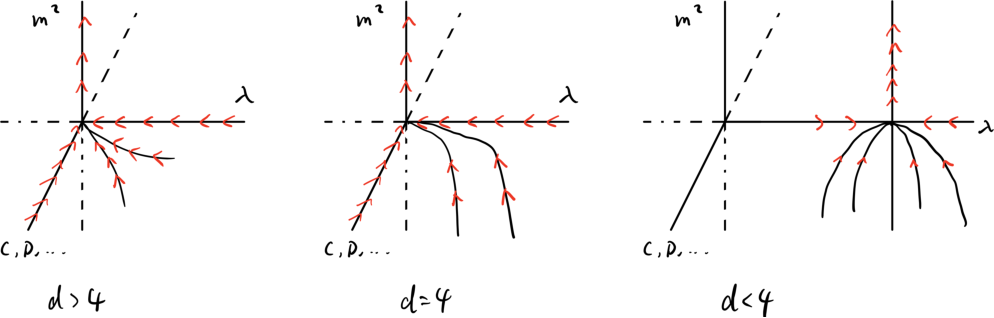
\includegraphics[width=0.8\linewidth]{./RG/RGFlow.pdf}
\end{align*}

\paragraph{Remarks}
\begin{itemize}
   \item for $d<4$ but "close", the new fixed point will be "close" to the free fixed point. Then perturbation theory still make sense. Could have stronly=coupled theories as a fixed point. More difficult, study exactly solvable models.
   \item $m^2 d^2$ im $\phi^4$ always relevant, diverges quickly, naturally $m \mapsto \Lambda$.Problems for theories with elementary scales (Higgs in Standard Model)
\end{itemize}


\end{document}
